\section{Obserwator stanu}
\subsection{Obserwator Luenbergera}
Po szczegółowej analizie zarejestrowanych przebiegów zauważono duży wpływ szumu kwantyzacji na jakość regulacji, szczególnie w przypadku prędkości kątowej wahadła wyliczanej przez iloraz różnicowy położenia wahadła w kolejnych chwilach czasu. W celu wygładzenia przebiegu prędkości zaprojektowano obserwator Luenbergera dla systemu zlinearyzowanego w taki sposób, aby błąd estymacji prędkości dostatecznie szybko zdążał do zera. Doświadczalnie wyznaczono odpowiednie ujemne wartości własne macierzy:
\begin{equation}  
eig(A-LC) = (-50,-1,-70,-80)
\end{equation} 
Zdecydowano się na obserwator pełnego rzędu, natomiast do regulatora podano jedynie estymacje stanów obarczonych największym błędem pomiarowym, prędkości wahadła i wózka.
\begin{figure}[H]
\centering
\label{fig:observ}
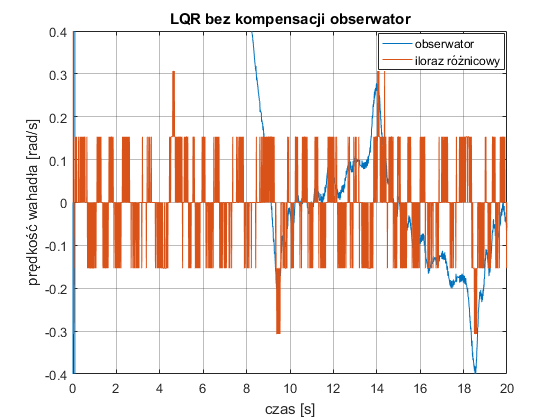
\includegraphics[width=14cm]{obrazy/pendulum/observ.png}
\caption{Estymator prędkości kątowej wahadła}
\end{figure}
Obserwator Luenbergera estymuje prędkość funkcją wyraźnie bardziej gładką niż to ma miejsce w przypadku obliczania ilorazu różnicowego. Niemniej jednak niedokładność modelu, a w największej mierze modelu tarcia, sprawia, że estymacja obarczona jest błędem, którego efekty są zauważalne w sposobie działania systemu.

Warto odnotować, że stabilizacja wahadła w pętli sprzężenia zwrotnego z sygnałami z obserwatora powiodła się, natomiast system wykazywał mniejszą odporność na zakłócenia.  
\subsection{Filtracja sygnału prędkości wahadła}
W celu zmniejszenia skutków niedoskonałości sygnału prędkości wahadła przetestowano szereg różnych podejść i eksperymentów. Wypróbowano filtr cyfrowy dolnoprzepustowy Czebyszewa II typu, którego zaletą jest stosunkowo wąskie pasmo przejściowe, a w odróżnieniu od typu I charakteryzuje się małymi zafalowaniami przebiegu w paśmie przepustowym. Biorąc pod uwagę częstotliwość taktowania algorytmu sterującego (100 Hz) przesuwano pasmo przepustowe w granicach 50-70 Hz, oraz pasmo zaporowe 60-95 Hz. O ile niewielka ingerencja w oryginalny sygnał nie wprowadzała zauważalnych zmian, o tyle duże tłumienia wprowadzały znaczące przesunięcie fazowe, które wpływało na zapasy stabilności systemu.

O wiele lepsze rezultaty dał filtr cyfrowy FIR o transmitancji:
\begin{equation}  
G(z) = 0.7 + 0.2z^{-1} + 0.1z^{-2}
\end{equation} 
natomiast jego zastosowania nie można uznać za przełomowe, ze względu na wprowadzane przesunięcie fazowe.

Kolejnym podejściem, które miało na celu zapewnienie mniej szarpanego działania wahadła było wprowadzenie filtru medianowego na sterowanie wychodzące z regulatora LQR. Pomysł okazał się nietrafiony, wahadło nie radziło sobie w przypadku wprowadzania zakłóceń.

Postanowiono wprowadzić predykcje prędkości na bazie dyskretnego modelu ARMAX, gdzie na podstawie ostatnich trzech próbek położenia wahadła, położenia wózka (sygnały obarczone najmniejszą niepewnością pomiarową) oraz sterowania podawanego na obiekt przewidywana byłaby prędkość wahadła oraz wózka w następnej chwili czasowej. Na tej podstawie możliwa stałaby się precyzyjniejsza rekonstrukcja prędkości. 